\section{Results and Discussion}

\begin{figure}[!htbp]

\begin{center}
\setlength\tabcolsep{1.5pt} % default value: 6pt
\medmuskip=-2mu
\thinmuskip=-2mu
\thickmuskip=-2mu
\nulldelimiterspace=-1pt
\scriptspace=0pt
\begin{tabular}{ | c || c c c | c c c | }
  \multicolumn{1}{c}{} & \multicolumn{3}{c}{Ecological Seeds} & \multicolumn{3}{c}{Mean Dominant ($\pm S.D.$)} \\
 \cline{2-7}
  \multicolumn{1}{c|}{} & \tiny{$P_{c} > P_{0,1}$} & \tiny{$P_0 > P_{c,1}$} & \tiny{$P_1 > P_{c,0}$} & \tiny{$P_{c} > P_{0,1}$} & \tiny{$P_0 > P_{c,1}$} & \tiny{$P_1 > P_{c,0}$}  \\
 \hline
 $n$ & 1 & 1 & 1 & 2 & 16 & 15  \\
 \hhline{|=||===|===|}
 $A_0$ & 0.00 & 1.00 & 1.00 & $0.09 \pm 0.13$ & $0.42 \pm 0.47$ & $0.27 \pm 0.41$ \\
 $A_1$ & 1.00 & 0.91 & 1.00 & $1.00 \pm  0.00$ & $0.99 \pm 0.02$ & $1.00 \pm 0.00$ \\
 \hline
 $P_{c}$ & 0.85 & 0.00 & 0.00 & $0.77 \pm 0.12$ & $0.05 \pm 0.04$ & $0.00 \pm 0.00$ \\
 $P_0$ & 0.07 & 1.00 & 0.00 & $0.13 \pm 0.09$ & $0.86 \pm 0.15$ & $0.00 \pm 0.00$ \\
 $P_1$ & 0.08 & 0.00 & 1.00 & $0.10 \pm 0.03$ & $0.09 \pm 0.15$ & $1.00 \pm 0.00$ \\
 \hline
 $C_0$ & 21.8 & 7.2 & 9.9 & $19.9 \pm 2.6$ & $10.4 \pm 2.5$ & $9.9 \pm 1.6$ \\
 $C_1$ & 101.2 & 274.2 & 238.2 & $93.7 \pm 10.6$ & $221.2 \pm 55.9$ & $244.0 \pm 23.0 $ \\
 \hline
 $E_{c}$ & 0.21 & 0.00 & 0.00 & $0.27 \pm 0.09$ & $0.02 \pm 0.05$ & $0.00 \pm 0.00$ \\
 $E_0$ & 1.21 & 30.1 & 0.00 & $1.3 \pm 0.1$ & $3.4 \pm 7.4$ & $0.046 \pm 0.13$ \\
 $E_1$ & 2.49 & 54.1 & 38.8 & $2.4 \pm 0.1$ & $29.4 \pm 16.9$ & $55.4 \pm 16.8$ \\
 \hline
 $M_{c}$ & 0.53 & 0.30 & 0.90 & $0.29 \pm 0.34$ & $0.35 \pm 0.40$ & $0.95 \pm 0.08$ \\
 $M_0$ & 1.00 & 0.00 & 1.00 & $0.86 \pm 0.20$ & $0.49 \pm 0.40$ & $0.67 \pm 0.46$ \\
 $M_1$ & 0.00 & 1.00 & 0.24 & $0.50 \pm 0.71$ & $0.51 \pm 0.47$ & $0.48 \pm 0.43$ \\
 \hline
 $S_0$ & 0.56 & 1.00 & 0.68 & $0.29 \pm 0.38$ & $0.44 \pm 0.46$ & $0.68 \pm 0.37$ \\
 $S_1$ & 1.00 & 0.84 & 0.71 & $0.50 \pm 0.71$ & $0.65 \pm 0.40$ & $0.45 \pm 0.40$ \\
 \hline
\end{tabular}
\end{center}
\caption{
Enumerations for genotypes used as seeds for ecological runs (left) and enumerations for mean values of the most abundant genotype at the end of evolutionary runs (right), both sorted by resource caching strategy.
}
\label{fig:genotypes}
\end{figure}


\begin{figure}[!htbp]
\begin{center}
\begin{subfigure}[b]{0.82\columnwidth}
  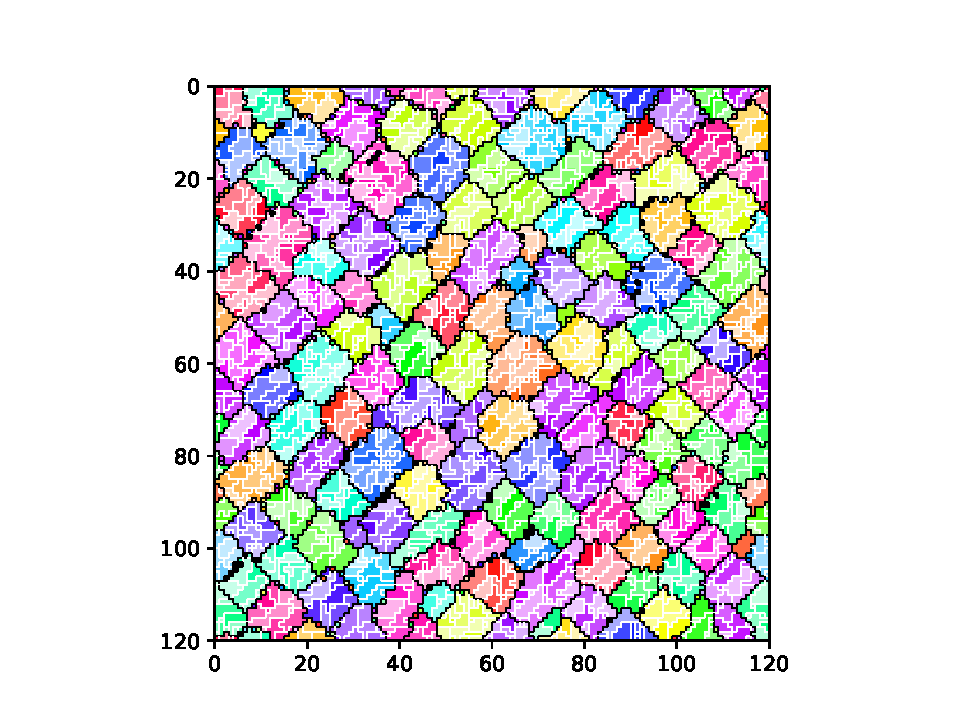
\includegraphics[width=\columnwidth,trim={2.5cm 0.5cm 2.5cm 1cm},clip]{img/ChannelMap_1022_update19500000}
  \caption{Mean $P_{c} = 0.77$, $P_0 = 0.089$, $P_1 = 0.14$; generation 20,475}
  \label{fig:ChannelMap_1022}
\end{subfigure}

\begin{subfigure}[b]{0.82\columnwidth}
  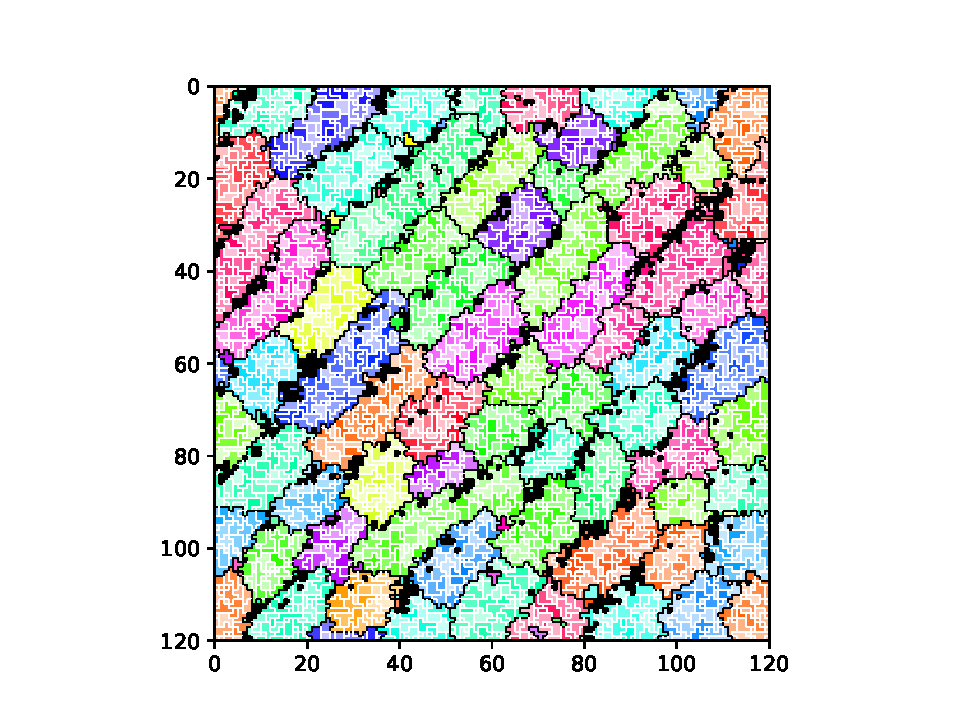
\includegraphics[width=\columnwidth,trim={2.5cm 0.5cm 2.5cm 1cm},clip]{img/ChannelMap_1041_update19500000}
  \caption{Mean $P_0 = 1.0$; generation 23,971}
  \label{fig:ChannelMap_1041}
\end{subfigure}

\begin{subfigure}[b]{0.82\columnwidth}
  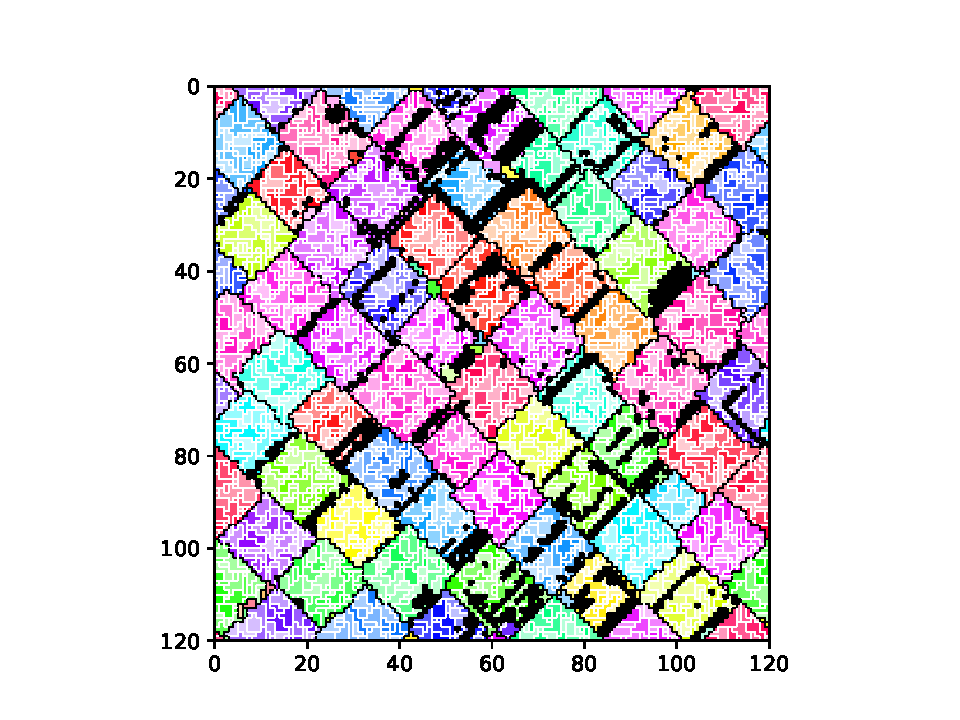
\includegraphics[width=\columnwidth,trim={2.5cm 0.5cm 2.5cm 1cm},clip]{img/ChannelMap_1008_update19500000}
  \caption{Mean $P_1 = 1.0$; generation 25,841}
  \label{fig:ChannelMap_1008}
\end{subfigure}

\caption{
State of same-channel level-zero and level-one signaling networks at the end of evolutionary runs where cell-level (\ref{fig:ChannelMap_1022}), zeroth-level (\ref{fig:ChannelMap_1041}), and first-level (\ref{fig:ChannelMap_1008}) individuality dominated.
Level-zero channels coded by HSV value are separated by white borders and level-one channels coded by HSV hue are separated by black borders.
}
\label{fig:outcome_grids}
\end{center}
\end{figure}


\begin{figure}[t]
\begin{center}
\begin{subfigure}[b]{0.5\columnwidth}
  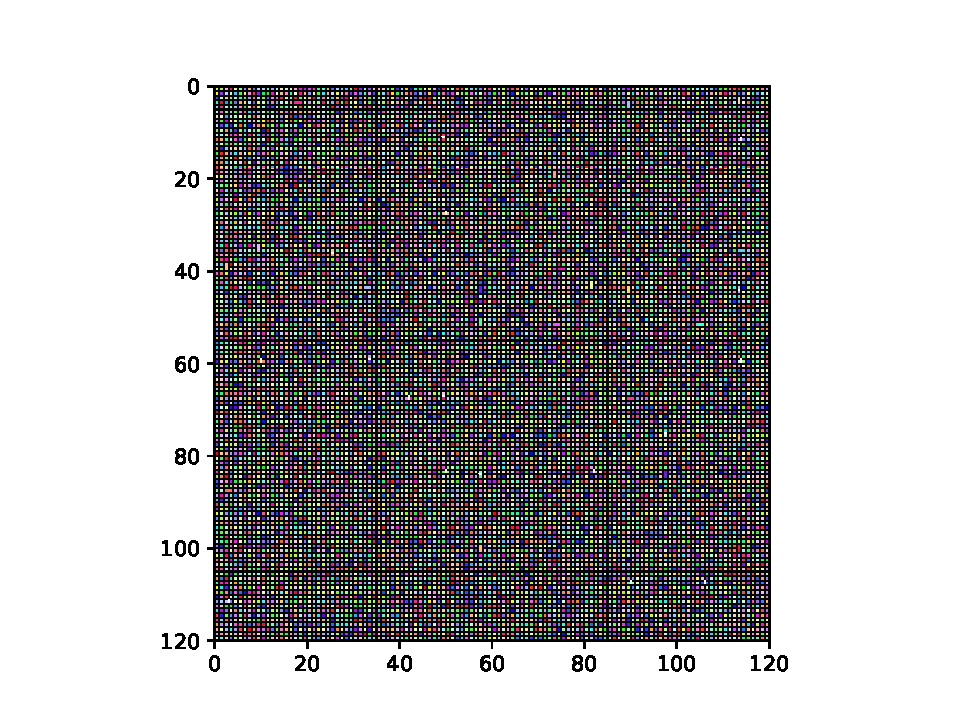
\includegraphics[width=\columnwidth,trim={2.5cm 0.5cm 2.5cm 1cm},clip]{img/ChannelMap_1011_update0}
  \caption{Update 0 (Generation 0)}
  \label{fig:ChannelMap_1011_update0}
\end{subfigure}%
\begin{subfigure}[b]{0.5\columnwidth}
  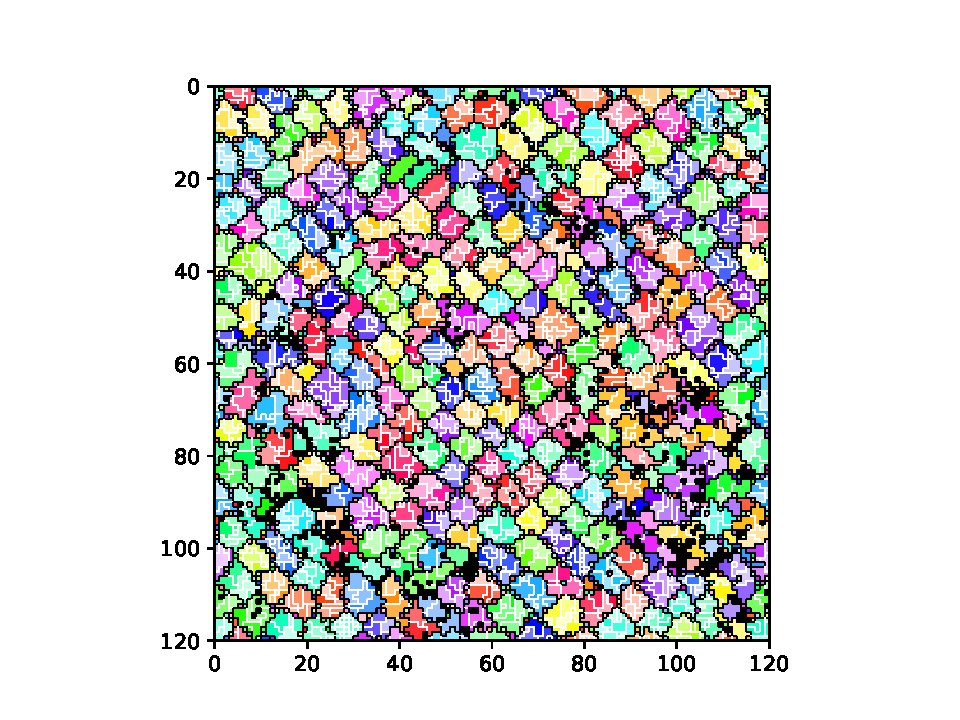
\includegraphics[width=\columnwidth,trim={2.5cm 0.5cm 2.5cm 1cm},clip]{img/ChannelMap_1011_update1000000}
  \caption{Update 1 million (Generation 927)}
  \label{fig:ChannelMap_1011_update1000000}
\end{subfigure}
\begin{subfigure}[b]{0.5\columnwidth}
  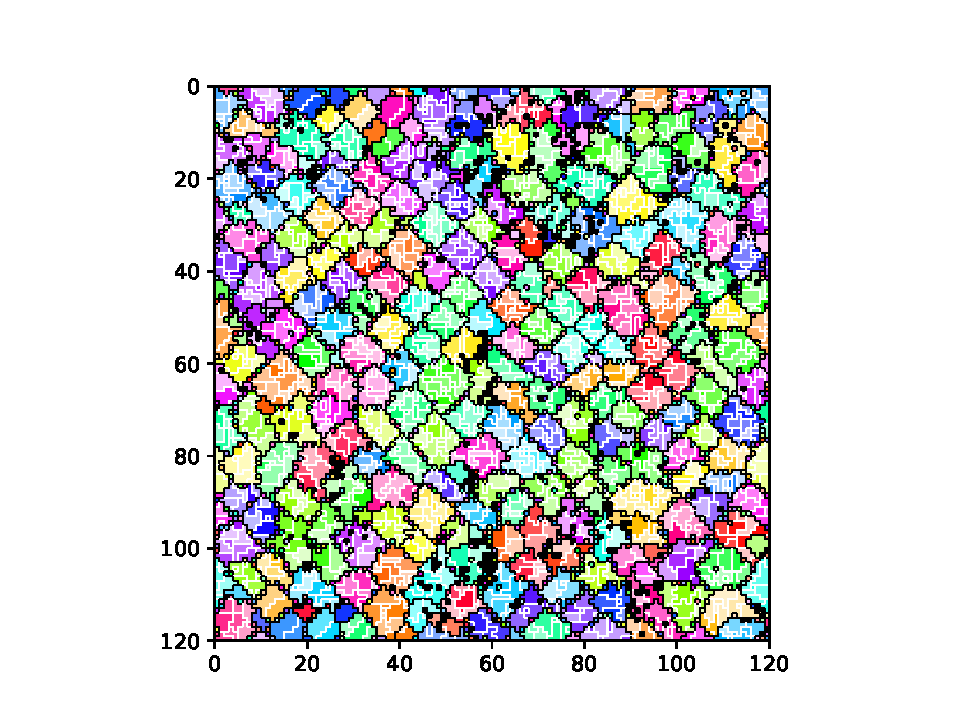
\includegraphics[width=\columnwidth,trim={2.5cm 0.5cm 2.5cm 1cm},clip]{img/ChannelMap_1011_update2000000}
  \caption{Update 2 million (Generation 1917)}
  \label{fig:ChannelMap_1011_update2000000}
\end{subfigure}%
\begin{subfigure}[b]{0.5\columnwidth}
  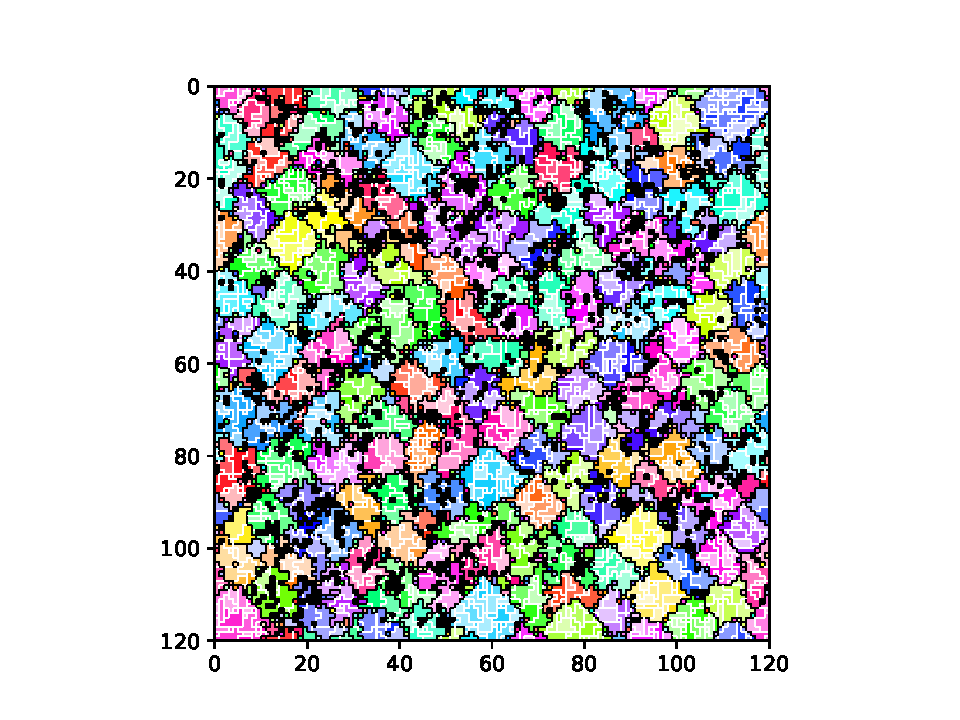
\includegraphics[width=\columnwidth,trim={2.5cm 0.5cm 2.5cm 1cm},clip]{img/ChannelMap_1011_update4000000}
  \caption{Update 4 million (Generation 4053)}
  \label{fig:ChannelMap_1011_update4000000}
\end{subfigure}
\begin{subfigure}[b]{0.5\columnwidth}
  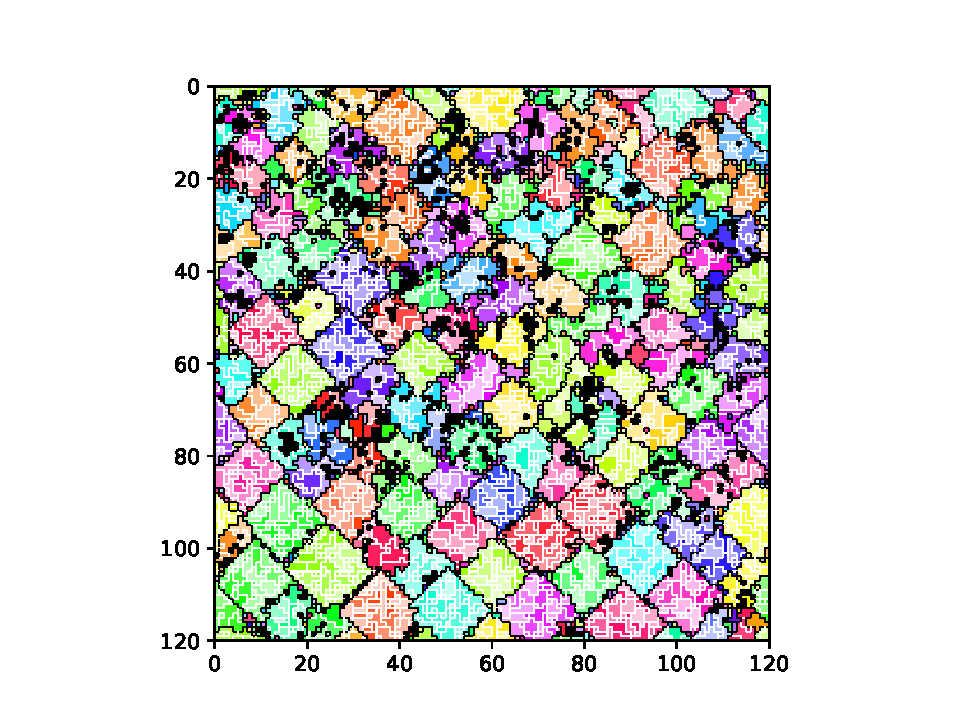
\includegraphics[width=\columnwidth,trim={2.5cm 0.5cm 2.5cm 1cm},clip]{img/ChannelMap_1011_update5000000}
  \caption{Update 5 million (Generation 5173)}
  \label{fig:ChannelMap_1011_update5000000}
\end{subfigure}%
\begin{subfigure}[b]{0.5\columnwidth}
  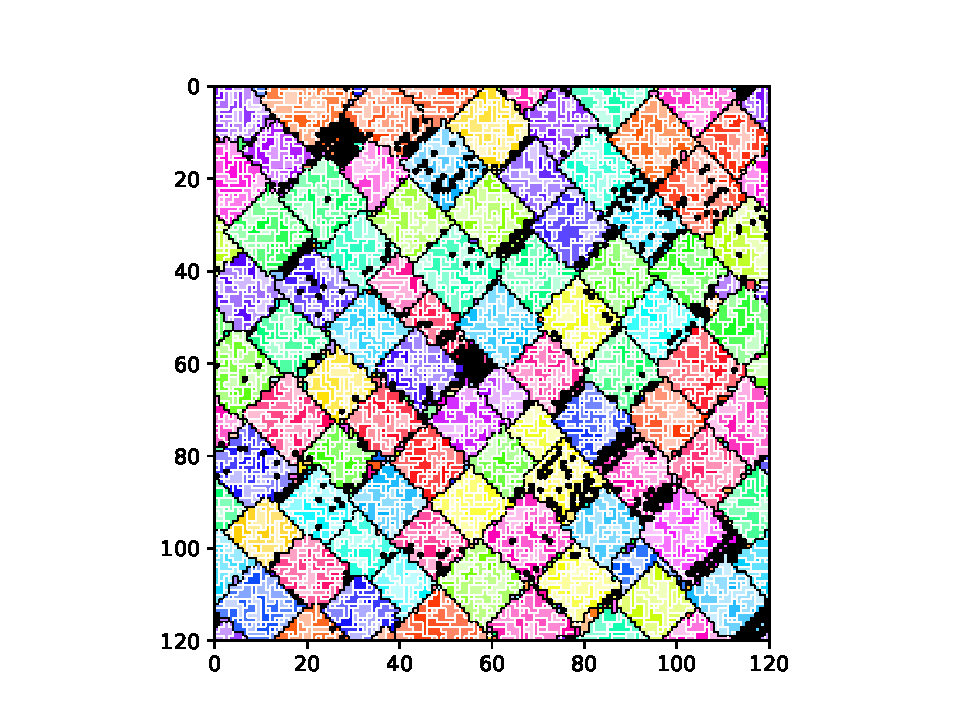
\includegraphics[width=\columnwidth,trim={2.5cm 0.5cm 2.5cm 1cm},clip]{img/ChannelMap_1011_update7000000}
  \caption{Update 7 million (Generation 7312)}
  \label{fig:ChannelMap_1011_update7000000}
\end{subfigure}
\caption{
Progression of of same-channel level-zero and level-one signaling networks states in an evolutionary run where population mean $P_1 > P_{c}, P_0$ evolved.
Level-zero channels coded by HSV value are separated by white borders and level-one channels coded by HSV hue are separated by black borders.
}
\label{fig:grid_progression}
\end{center}
\end{figure}


\begin{figure}[t]
\begin{center}

\begin{subfigure}[b]{0.5\columnwidth}
  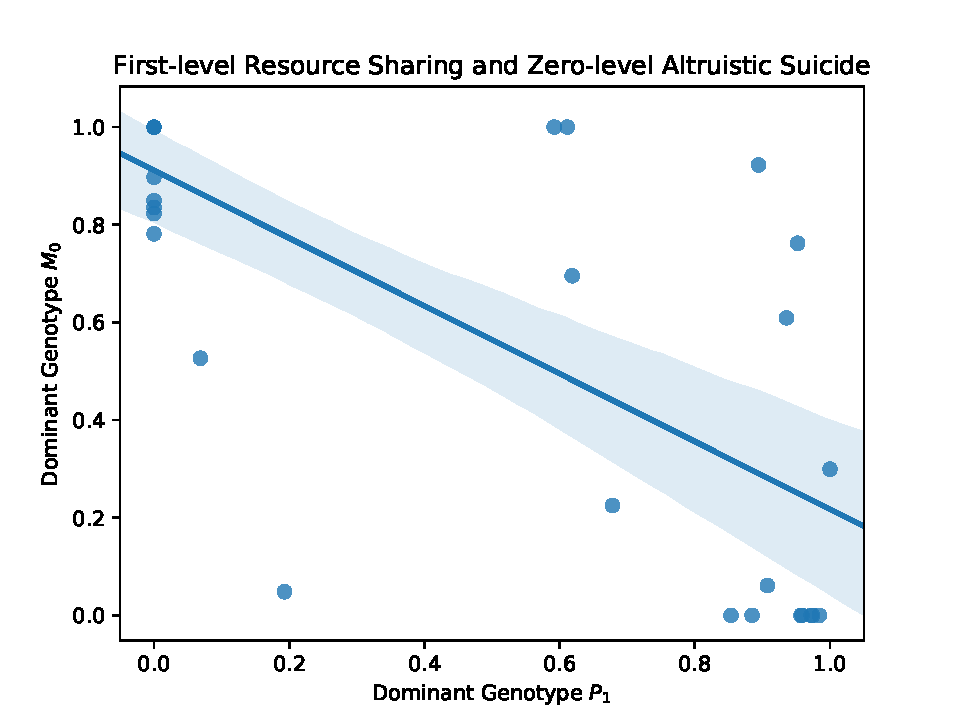
\includegraphics[width=\columnwidth]{img/champion_res_pool1_vs_champion_damage_suicide0}
  \caption{
  Correlation plot of dominant genotype $P_0$ and dominant genotype $M_{self}$.
  }
  \label{fig:champion_res_pool1_vs_champion_damage_suicide0}
\end{subfigure}%
\begin{subfigure}[b]{0.5\columnwidth}
  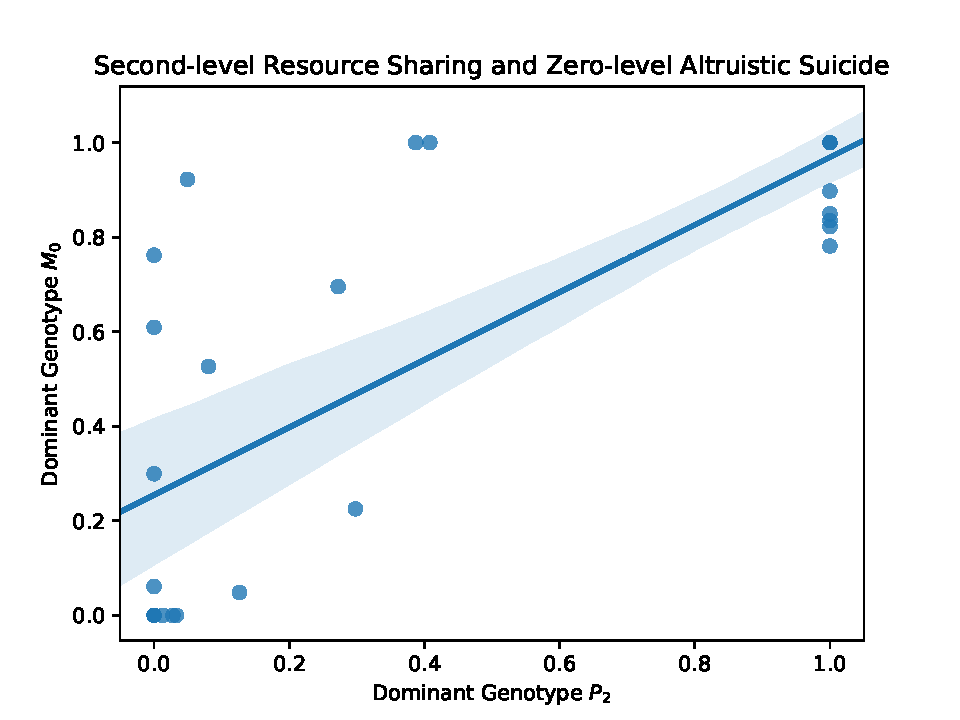
\includegraphics[width=\columnwidth]{img/champion_res_pool2_vs_champion_damage_suicide0}
  \caption{
  Correlation plot of dominant genotype $P_1$ and dominant genotype $M_{self}$.
  }
  \label{fig:champion_res_pool2_vs_champion_damage_suicide0}
\end{subfigure}

\caption{
Plots of dominant resource caching strategies and dominant apoptosis strategies.
A bootstrapped 95\% confidence interval for the fit is shaded.
}
\label{fig:damage_suicide}
\end{center}
\end{figure}


\begin{figure}[t]
\begin{center}

\begin{subfigure}[b]{0.5\columnwidth}
  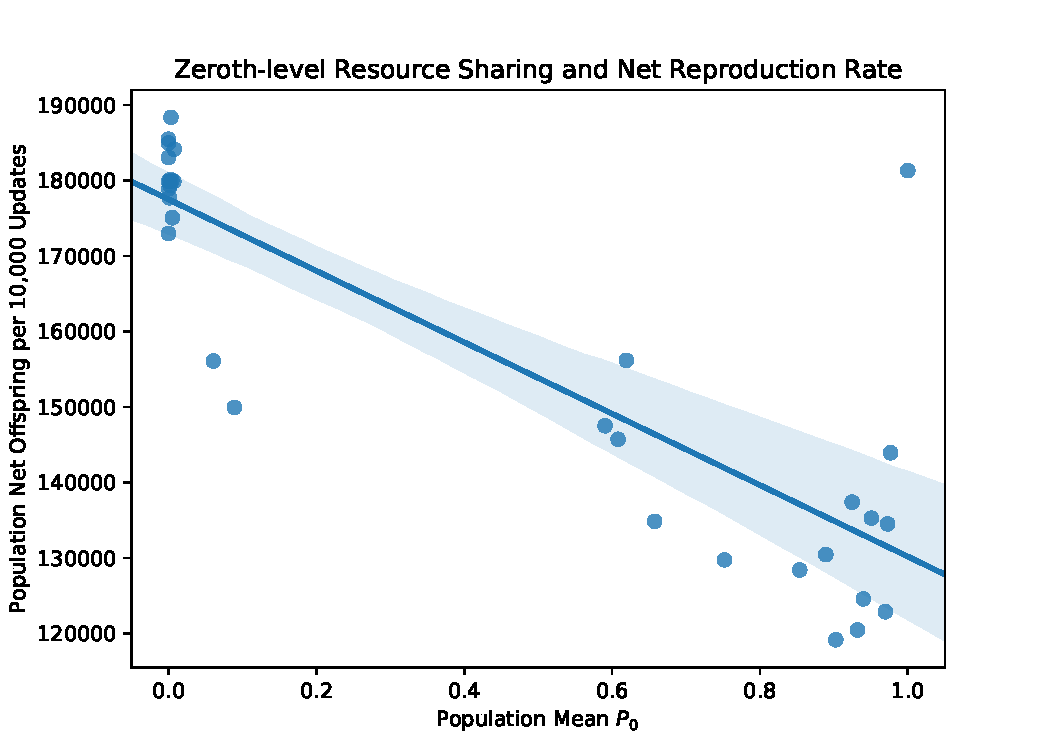
\includegraphics[width=\columnwidth]{img/mean_res_pool1_vs_net_reproduction}
  \caption{
  Correlation plot of population mean $P_0$ and population net reproduction rate.
  }
  \label{fig:mean_res_pool1_vs_net_reproduction}
\end{subfigure}%
\begin{subfigure}[b]{0.5\columnwidth}
  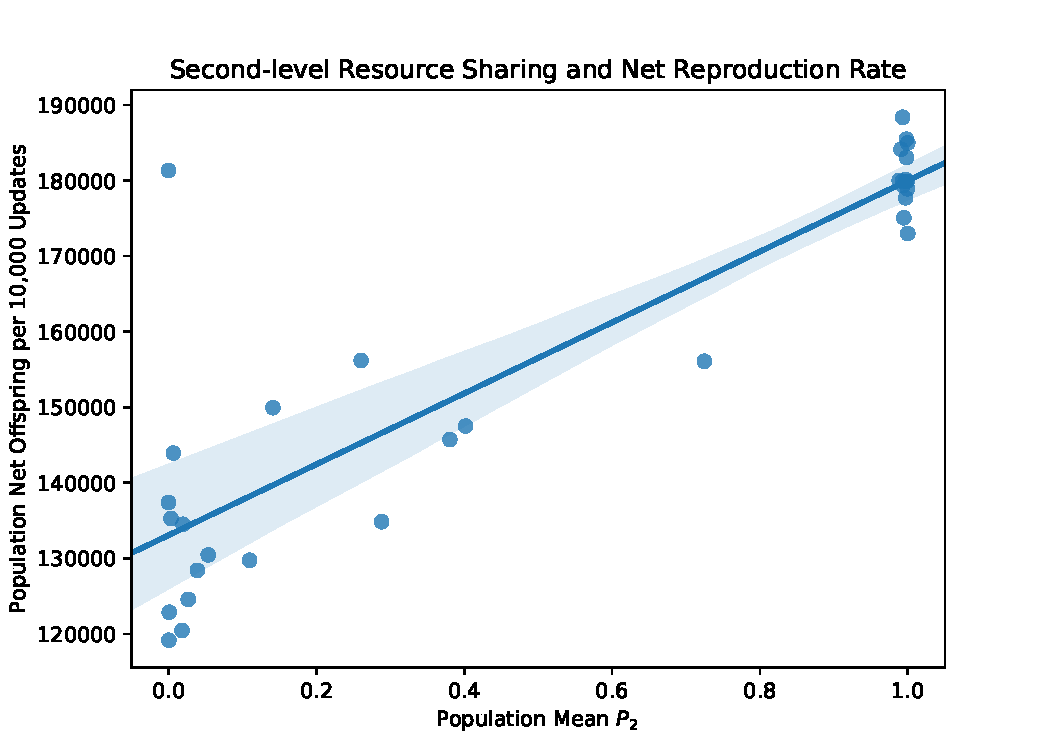
\includegraphics[width=\columnwidth]{img/mean_res_pool2_vs_net_reproduction}
  \caption{
  Correlation plot of population mean $P_1$ and population net reproduction rate.
  }
  \label{fig:mean_res_pool2_vs_net_reproduction}
\end{subfigure}
\caption{
Mean resource caching strategies and net reproduction rate across populations.
A bootstrapped 95\% confidence interval for the fit is shaded.
}
\label{fig:net_reproduction}
\end{center}
\end{figure}


\begin{figure}[!htbp]
\begin{center}

\begin{subfigure}[b]{0.5\columnwidth}
  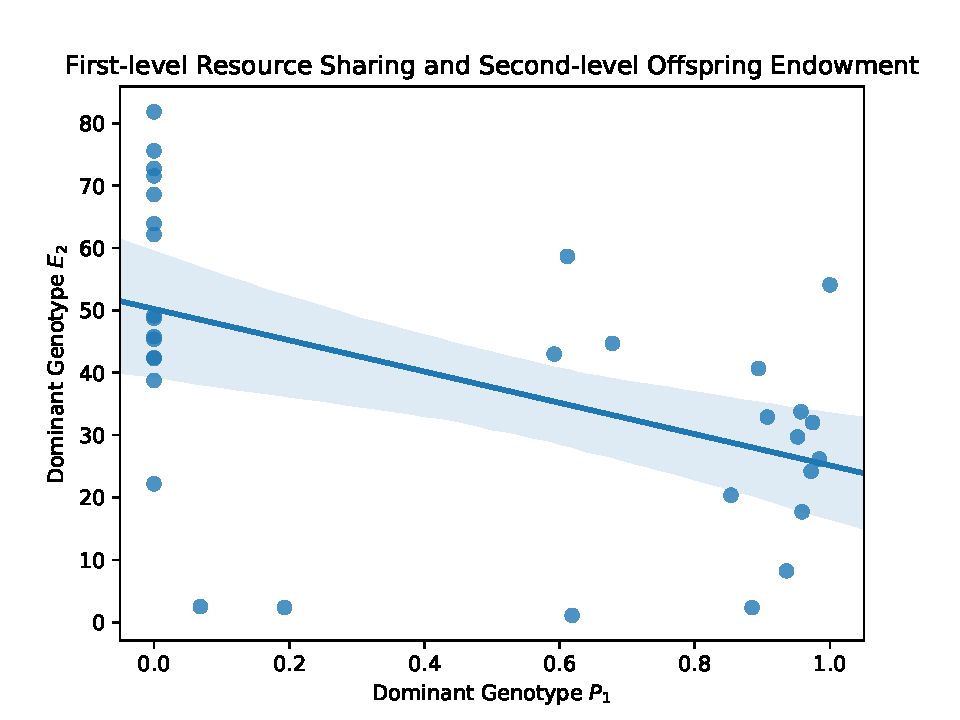
\includegraphics[width=\columnwidth]{img/champion_res_pool1_vs_champion_endowment2}
  \caption{
  Correlation plot of dominant genotype $P_0$ and dominant genotype $E_1$.
  }
  \label{fig:champion_res_pool1_vs_champion_endowment2}
\end{subfigure}%
\begin{subfigure}[b]{0.5\columnwidth}
  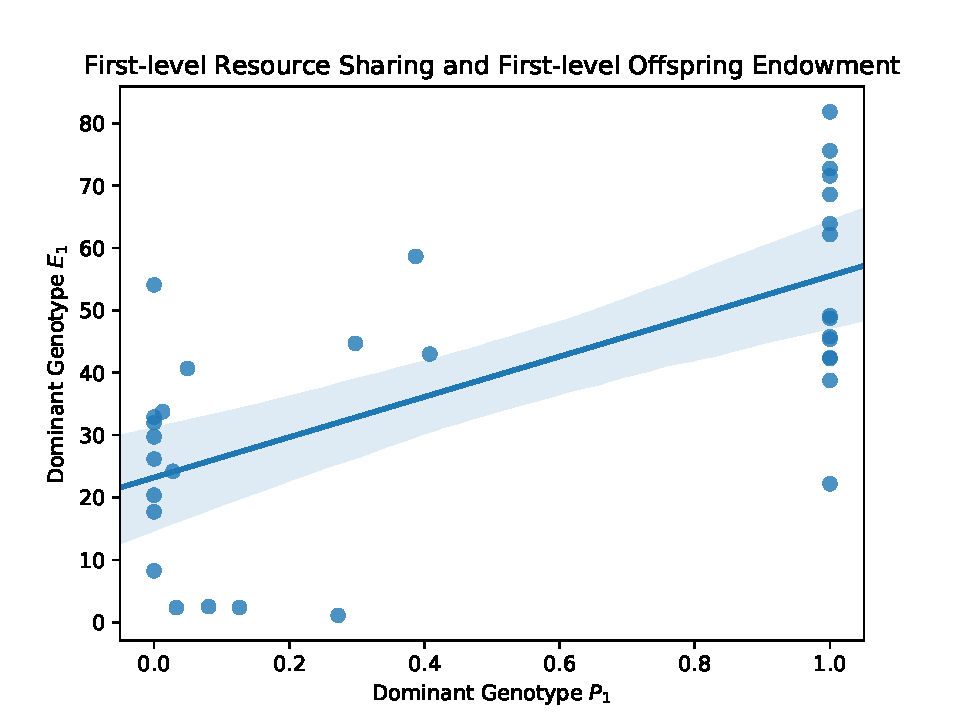
\includegraphics[width=\columnwidth]{img/champion_res_pool2_vs_champion_endowment2}
  \caption{
  Correlation plot of dominant genotype $P_1$ and dominant genotype $E_1$.
  }
  \label{fig:champion_res_pool2_vs_champion_endowment2}
\end{subfigure}

\caption{
Plots of dominant resource caching strategies and dominant propagule endowment strategies.
A bootstrapped 95\% confidence interval for the fit is shaded.
}
\label{fig:endowment}
\end{center}
\end{figure}


Zeroth-, first-, and second- level individuals were all observed at update 19.5 million (~ generation TODO) in different runs of our evolutionary simulation.
The criteria used to discern these outcomes are described below.
Figure \ref{fig:outcome_grids} shows the level-zero and level-one signaling networks at the end of runs where zero-, first-, and second-level individuality evolved, respectively.
Figure \ref{fig:grid_progression} shows a time series of signaling network snapshots in an evolutionary run where second-level individuality evolved.
Zeroth-level individuals appear to form with comparatively large level zero signaling networks that are arranged into roughly globular level-one signaling networks.
% @CAO: What does "roughly globular" mean?  Perhaps this should be "amorphous"?
First-level individuals appear to form elongated cigar-shaped level one amalgamations of diverse level-zero networks.
Second-level individuals appear to form highly regular diamond-shaped one- level amalgamations of diverse level zero networks.

Figure \ref{fig:genotypes} describes predominant genotypes observed at the end of evolutionary simulation.
With a single exception, nearly all evolved genotypes had $A_1$ fixed at or very near $1.0$ (i.e. population mean $A_1 \geq 0.993$) .
So, reproduction over cells sharing the same level-one channel was near-universally avoided;
genotypes evolved so that organisms surrendered their ability to reproduce when they were located at the interior of level one same-channel signaling networks. % (at least as long as they remained at the interior of the network).
%We confirmed that reproductive abstention indeed occurred in our system as expected by directly logging it.

However, a variety of resource-caching strategies evolved.
Most-abundant genotypes at the end of evolutionary runs included strategies where resource was primarily cached in an organism's individual stockpile (i.e. $P_{c} > P_0, P_1$), strategies where resource was primarily cached in an organism's level-zero signaling network's pool (i.e. $P_0 > P_{c}, P_1$), and strategies where resource was primarily cached in an organism's level-one signaling network's pool (i.e. $P_1 > P_{c}, P_0$).
% Should we change each of the >'s above into >> to indicate MUCH greater than?  As long as it's true from SOME runs, it doesn't need to be frequent.
%Among 33 trials, at update 19.5 million predominant genotypes with $P_{c} > P_0, P_1$ were observed in two replicates, predominant genotypes with $P_0 > P_{c}, P_1$ were observed in 16 replicates, and predominant genotypes with $P_1 > P_{c}, P_0$ were observed in 15 replicates.
Among 33 trials, selfish low-level individuals dominated by the end of two replicates, level-zero resource-sharing dominated in 16 replicates, and level-one resource sharing dominated in 15 replicates.
%@CAO: I think the above will be easier for readers to digest.  I'm not sure why you focused on 19.5 million (I'm assuming it has to do with data collection), but I think it's a fine point to count as "by the end"  I also wouldn't include the below since it's basically the same timepoint; you could just update the numbers above to 1,16,16 if you want.
%A related measure, among populations at update 19.99 million mean $P_{c} > P_0, P_1$ was observed in one replicate, mean $P_0 > P_{c}, P_1$ was observed in 16 replicates, and mean $P_1 > P_{c}, P_1$ was observed in 16 replicates.

Given the near-ubiquitous nature of cooperation with regard to reproductive division of labor at the level one same-channel signaling network, it was on this basis of resource caching strategy that distinctions between zeroth-, first-, and second- level individuality was drawn.
(The single predominant genotype with $A_1 = 0.91$ had $P_0 = 1.0$, so was not sharing resource on the level one same-channel resource pool).
% @CAO: I'm not sure where this final parenthetical came from.  I take it this is the single "selfish" individual in the second example above?

Next, we wanted to compare zeroth-, first-, and second-level individuals to determine which genotype was the most fit in the DISHTINY environment.
We ran ecological competitions between the the dominant genotypes from the run with greatest mean $P_{c}$, the run with greatest mean $P_0$, and the run with greatest mean $P_1$.
Out of 191 trials performed, by update 1.5 million, fixation was reached.  % @CAO: Should this be "a single genotype fixed in each case." or something along those lines?
The zeroth-level individuality genotype dominated in one trial, the first-level individuality genotype dominated in 12 trials, and the second-level individuality genotype dominated in 178 trials.
These results suggest that in the absence of mutation, second-level individuals tend to exhibit greater fitness than first- and zero-th level individuals ($p < 0.0001$; RR 2.8; two-tailed exact test).

In this comparison, however, higher-level individuality likely benefited from eliminated the problem of somatic mutation.
To assess the relative fitness of first- and second-level individuals without mutation disabled, we examined the relationship between mean $P_0$ and $P_1$ and the rate of cellular reproduction at the end of each of the 33 replicate evolutionary trials performed.
We observed a significant negative correlation between mean $P_0$ and cellular reproduction rate ($p < 0.0001$; bootstrap test; Figure \ref{fig:mean_res_pool1_vs_net_reproduction}) and a significant positive correlation between mean $P_1$ and cellular reproduction rate ($p < 0.0001$; bootstrap test; Figure \ref{fig:mean_res_pool2_vs_net_reproduction}).
This result suggests that second-level individuals tend to collect resource more effectively than first-level individuals.
We did not test correlation between $P_{c}$ and due to the small number of outcomes where elevated $P_{c}$ was observed.

With the viability of zero-, first-, and second-level individuality in the DISHTINY environment --- and the greater relative fitness of second-level individuality --- established, we were also interested in probing the strategies employed by zero-, first-, and second-level individuals beyond resource caching and reproductive deferment.
To assess whether higher-level individuals employed apoptosis to mitigate somatic mutation, we examined the relationship between dominant genotype $P_0$ and $P_1$ and dominant genotype $M_{c}$ at update 19.5 million in the 33 replicate evolutionary trials performed.
We observed a significant negative correlation between dominant genotype $P_0$ and $M_{c}$ ($p < 0.0001$; bootstrap test; Figure \ref{fig:champion_res_pool1_vs_champion_damage_suicide0}) and a significant positive correlation between dominant genotype $P_1$ and $M_{c}$ ($p < 0.0001$; bootstrap test; Figure \ref{fig:champion_res_pool2_vs_champion_damage_suicide0}).
Notably, no genotype encoding second-level individuality was observed with $M_{c} < 0.5$.
This result suggests that second-level individuals, in particular, relied on apoptosis to mitigate somatic mutation, perhaps due to their much larger scale compared to first- and zeroth-level individuals.

To assess whether higher-level individuals provided larger resource enowments to their propagules (offspring sharing neither the level zero nor the level one channel ID with the parent), we examined the relationship between dominant genotype $P_0$ and $P_1$ and dominant genotype $E_1$ at update 19.5 million in the 33 replicate evolutionary trials performed.
We observed a significant negative correlation between dominant genotype $P_0$ and $E_1$ ($p < 0.001$; bootstrap test; Figure \ref{fig:champion_res_pool1_vs_champion_endowment2}) and a significant positive correlation between dominant genotype $P_1$ and $E_1$ ($p <  0.0001$; bootstrap test; Figure \ref{fig:champion_res_pool2_vs_champion_endowment2}).
Second-level individuals might provide larger endowments to propagules simply due to a greater capacity to collect resource or perhaps because of stronger selection for well-endowed offspring when competing against other second-level individuals.
%@CAO should we speculate why we believe it's the second of these options?
